\documentclass[../../main.tex]{subfiles}
\begin{document}

{\bf [解]}
\paragraph{(1)}
与えられた関数
\begin{align}
 f_n(x)=a_n(x-n)(n+1-x)=-a_n(x-n)(x-n-1) \label{eq:1}
\end{align}
について考える．一階微分は
\begin{align}
 f_n'(x)=-a_n\{2x-(2n+1)\} \label{eq:2}
\end{align}
である．

$y=f_n(x)$と$y=e^{-x}$が$x=\alpha_n$で接するとすると，これら二曲線の$y$座標と一階微分が同じである．従って
\begin{align}
 &\begin{cases}
  f_n(\alpha_n) = e^{-\alpha_n} \\
  f'_n(\alpha_n) = -e^{-\alpha_n}
 \end{cases} \\
 &\begin{cases}\\
  -a_n(\alpha_n-n)(\alpha_n-n-1)&=e^{-\alpha_n} \\
  -a_n\{2\alpha_n-(2n+1)\}&=-e^{-\alpha_n} 
  \end{cases} \label{eq:3}
\end{align}
である．$e^{-\alpha_n}$を消去すると
\begin{align}
 -a_n(\alpha_n-n)(\alpha_n-n-1) = a_n\{2\alpha_n-(2n+1)\} 
\end{align}
$a_n\neq 0$で両辺わって
\begin{align}
 -(\alpha_n-n)(\alpha_n-n-1)=2\alpha_n-2n-1
\end{align}
である．さらに新しく
\begin{align}
 \beta_n = \alpha_n-n \label{eq:4}
\end{align}
とおくと，
\begin{align}
 &-\beta_n(\beta_n-1)=2\beta_n-1 \\
 & \beta_n^2+\beta_n-1=0 \\
 & \beta_n=\dfrac{-1\pm\sqrt{5}}{2} \label{eq:5}
\end{align}
である．

さてここで，$a_n>0,\ e^{-\alpha_n}>0$より\cref{eq:3}の第一式から
\begin{align}
 &(\alpha_n-n)(\alpha_n-n-1)<0 \\
 &\beta_n(\beta_n-1)<0 \\
 &0<\beta_n<1 
\end{align}
である．

これをみたすのは\cref{eq:5}のうち複合正の$\beta=\dfrac{-1+\sqrt{5}}{2}$のみだから\cref{eq:4}より
\begin{align}
\alpha_n=n+\dfrac{-1+\sqrt{5}}{2}\qquad(n<\alpha_n<n+1) \label{eq:6}
\end{align} 
である．

\cref{eq:3}の第二式に代入して
\begin{align}
 a_n
  &=\dfrac{e^{-\alpha_n}}{2\alpha_n-2n-1} \\
  &=\dfrac{e^{-\alpha_n}}{2\beta_n-1} \\
  &=\dfrac{e^{-\alpha_n}}{(-1+\sqrt{5}) -1} \quad (\because\text{\cref{eq:5}})\\
  &=\dfrac{e^{-\alpha_n}}{-2+\sqrt{5}} \\
  &=(2+\sqrt{5})\,e^{-n-\frac{-1+\sqrt{5}}{2}} \\
  &=(2+\sqrt{5})\,e^{\frac{1-\sqrt{5}}{2}}\,e^{-n} \label{eq:7}
\end{align}
である．


\paragraph{(2)}

簡単のため
\begin{align}
 K=(2+\sqrt{5})e^{\frac{1-\sqrt{5}}{2}} \label{eq:8}
\end{align}
とおくと\cref{eq:7}より
\begin{align}
 a_n=Ke^{-n} \label{eq:9}
\end{align}
である．


\begin{figure}[htb]
\centering
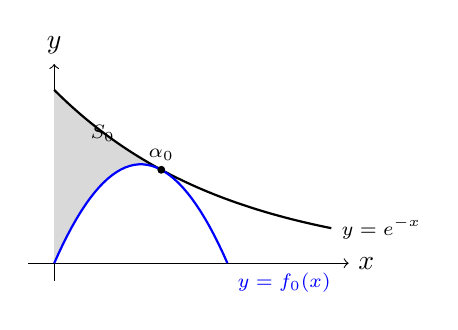
\begin{tikzpicture}[scale=2.2]
  % 座標軸
  \draw[->] (-0.15,0) -- (1.7,0) node[right]{$x$};
  \draw[->] (0,-0.1) -- (0,1.15) node[above]{$y$};
  % S_0: y=f_0(x), y=e^{-x} と y軸で囲まれる部分 (alpha_0=(-1+sqrt5)/2, a_0=K)
  \fill[gray!30] (0,0) -- (0,1) -- plot[domain=0:0.618,samples=30] (\x,{exp(-\x)}) -- plot[domain=0.618:0,samples=30] (\x,{2.2836*\x*(1-\x)}) -- cycle;
  \draw[thick,domain=0:1.6,samples=60] plot (\x,{exp(-\x)}) node[right]{\scriptsize$y=e^{-x}$};
  \draw[thick,blue,domain=0:1,samples=40] plot (\x,{2.2836*\x*(1-\x)}) node[below right]{\scriptsize$y=f_0(x)$};
  \node at (0.28,0.75) {\scriptsize$S_0$};
  \filldraw (0.618,{exp(-0.618)}) circle(0.55pt) node[above]{\scriptsize$\alpha_0$};
\end{tikzpicture}
\caption{$S_0$：$y=f_0(x)$，$y=e^{-x}$と$y$軸で囲まれる部分}
\end{figure}

\begin{figure}[htb]
\centering
\begin{tikzpicture}[scale=2.4, >=stealth, every node/.style={font=\small}]

  % --- 1. パラメータ設定と解析計算 ---
  % 基準となる n の値 (図示用として n = 1 を基準に設定)
  \def\n{1.0}
  
  % 定数 K = (2 + \sqrt{5}) * e^{(1 - \sqrt{5})/2} \approx 2.2836
  \pgfmathsetmacro{\K}{(2.0 + sqrt(5.0)) * exp((1.0 - sqrt(5.0)) / 2.0)}
  % \beta = (-1 + \sqrt{5}) / 2 \approx 0.61803
  \pgfmathsetmacro{\betaVal}{(-1.0 + sqrt(5.0)) / 2.0}
  
  % 接点 \alpha_{n-1}, \alpha_n
  \pgfmathsetmacro{\alphaPrev}{\n - 1.0 + \betaVal}
  \pgfmathsetmacro{\alphaCurr}{\n + \betaVal}
  
  % 係数 a_{n-1}, a_n
  \pgfmathsetmacro{\aPrev}{\K * exp(-(\n - 1.0))}
  \pgfmathsetmacro{\aCurr}{\K * exp(-\n)}

  % --- 2. 領域 S_n の斜線ハッチング ---
  % 上側境界: y = e^{-x} (\alpha_{n-1} から \alpha_n)
  % 下側境界: y = f_n(x) (\alpha_n から n) および y = f_{n-1}(x) (n から \alpha_{n-1})
  \fill[pattern=north east lines, pattern color=black!40]
    plot[domain=\alphaPrev:\alphaCurr, samples=40] (\x, {exp(-\x)})
    -- plot[domain=\alphaCurr:\n, samples=30] (\x, {-\aCurr * (\x - \n) * (\x - \n - 1.0)})
    -- plot[domain=\n:\alphaPrev, samples=30] (\x, {-\aPrev * (\x - \n + 1.0) * (\x - \n)})
    -- cycle;

  % --- 3. 補助線（点線） ---
  \draw[dashed, gray!70] (\alphaPrev, 0) -- (\alphaPrev, {exp(-\alphaPrev)});
  \draw[dashed, gray!70] (\alphaCurr, 0) -- (\alphaCurr, {exp(-\alphaCurr)});

  % --- 4. 座標軸 ---
  \draw[->, thick] ({\n - 1.4}, 0) -- ({\n + 1.5}, 0) node[right] {$x$};
  \draw[->, thick] ({\n - 1.3}, -0.3) -- ({\n - 1.3}, 1.2) node[above] {$y$};

  % --- 5. 曲線描画 ---
  % 指数関数 y = e^{-x}
  \draw[very thick, red!80!black, domain={\n - 1.2}:{\n + 1.4}, samples=60] 
    plot (\x, {exp(-\x)}) node[above right] {$y = e^{-x}$};

  % 放物線 y = f_{n-1}(x)
  \draw[very thick, blue!80!black, domain={\n - 1.15}:{\n + 0.15}, samples=50] 
    plot (\x, {-\aPrev * (\x - \n + 1.0) * (\x - \n)}) node[left, font=\footnotesize] {$y = f_{n-1}(x)$};

  % 放物線 y = f_n(x)
  \draw[very thick, blue!80!black, domain={\n - 0.25}:{\n + 1.15}, samples=50] 
    plot (\x, {-\aCurr * (\x - \n) * (\x - \n - 1.0)}) node[below left, font=\footnotesize] {$y = f_n(x)$};

  % --- 6. 軸上の目盛りラベル ---
  \node[below] at ({\n - 1.0}, 0) {$n-1$};
  \node[below] at (\n, 0) {$n$};
  \node[below] at ({\n + 1.0}, 0) {$n+1$};
  \node[below] at (\alphaPrev, 0) {$\alpha_{n-1}$};
  \node[below] at (\alphaCurr, 0) {$\alpha_n$};

  % --- 7. プロット点 ---
  % x軸との交点
  \fill ({\n - 1.0}, 0) circle (0.7pt);
  \fill (\n, 0) circle (0.7pt);
  \fill ({\n + 1.0}, 0) circle (0.7pt);

  % 接点
  \fill[red!80!black] (\alphaPrev, {exp(-\alphaPrev)}) circle (0.9pt);
  \fill[red!80!black] (\alphaCurr, {exp(-\alphaCurr)}) circle (0.9pt);

  % --- 8. 引出線付き領域ラベル S_n ---
  \draw[->, thick] ({\n + 0.3}, 0.8) to[out=190, in=80] ({\n + 0.05}, 0.42);
  \node[above right, font=\bfseries] at ({\n + 0.25}, 0.75) {$S_n$};

\end{tikzpicture}
\caption{一般の $n$ に対する領域 $S_n$（斜線部）と曲線 $y=e^{-x}, y=f_{n-1}(x), y=f_n(x)$}
\end{figure}

\begin{figure}[htb]
\centering
\begin{tikzpicture}[scale=2.2, yscale=4.0, >=stealth, every node/.style={font=\small}]

  % --- 1. 定数・解析的パラメータ設定 ---
  % K = (2 + \sqrt{5}) * e^{(1 - \sqrt{5})/2} \approx 2.2836
  \pgfmathsetmacro{\K}{(2.0 + sqrt(5.0)) * exp((1.0 - sqrt(5.0)) / 2.0)}
  % \beta = (-1 + \sqrt{5}) / 2 \approx 0.61803
  \pgfmathsetmacro{\betaVal}{(-1.0 + sqrt(5.0)) / 2.0}
  
  % 図示する n の値 (n = 3 として 0 から \alpha_3 までを図示)
  \def\n{3}
  \pgfmathsetmacro{\alphaEnd}{\n + \betaVal}

  % 各区間の係数 a_k
  \pgfmathsetmacro{\aZero}{\K * exp(0.0)}
  \pgfmathsetmacro{\aOne}{\K * exp(-1.0)}
  \pgfmathsetmacro{\aTwo}{\K * exp(-2.0)}
  \pgfmathsetmacro{\aThree}{\K * exp(-3.0)}

  % --- 2. 面積 T_n = \sum_{k=0}^n S_k の斜線塗りつぶし (x = 0 から x = \alpha_n) ---
  % 上側境界: y = e^{-x} (0 <= x <= \alpha_n)
  % 下側境界: 各放物線 y = f_k(x) (0 <= x <= \alpha_n)
  \fill[pattern=north east lines, pattern color=black!40]
    (0,0) -- (0,1)
    -- plot[domain=0:\alphaEnd, samples=60] (\x, {exp(-\x)})
    -- plot[domain=\alphaEnd:3, samples=20] (\x, {-\aThree * (\x - 3) * (\x - 4)})
    -- plot[domain=3:2, samples=20] (\x, {-\aTwo * (\x - 2) * (\x - 3)})
    -- plot[domain=2:1, samples=20] (\x, {-\aOne * (\x - 1) * (\x - 2)})
    -- plot[domain=1:0, samples=20] (\x, {-\aZero * \x * (\x - 1)})
    -- cycle;

  % --- 3. 座標軸 ---
  \draw[->, thick] (-0.3, 0) -- (4.6, 0) node[right] {$x$};
  \draw[->, thick] (0, -0.2) -- (0, 1.45) node[above] {$y$};
  \node[below left] at (0,0) {$O$};

  % --- 4. 曲線群の描画 ---
  % (i) 指数関数 y = e^{-x}
  \draw[very thick, red!80!black, domain=-0.2:4.3, samples=70] 
    plot (\x, {exp(-\x)}) node[right] {$y = e^{-x}$};

  % (ii) 各放物線 y = f_k(x)
  \draw[very thick, blue!80!black, domain=-0.05:1.05, samples=30] 
    plot (\x, {-\aZero * \x * (\x - 1)});
  \draw[very thick, blue!80!black, domain=0.95:2.05, samples=30] 
    plot (\x, {-\aOne * (\x - 1) * (\x - 2)});
  \draw[very thick, blue!80!black, domain=1.95:3.05, samples=30] 
    plot (\x, {-\aTwo * (\x - 2) * (\x - 3)});
  \draw[very thick, blue!80!black, domain=2.95:4.05, samples=30] 
    plot (\x, {-\aThree * (\x - 3) * (\x - 4)});

  % 放物線群の代表ラベル
  \draw[->, thick, blue!80!black] (2.7, 0.75) to[out=200, in=80] (2.15, 0.22);
  \node[above right, blue!80!black, font=\normalsize] at (2.4, 0.7) {$y = f_k(x)$};

  % --- 5. 終端 x = \alpha_n の境界線（点線と接点） ---
  \draw[dashed, thick, gray!80!black] (\alphaEnd, 0) -- (\alphaEnd, {exp(-\alphaEnd)});
  % \fill[red!80!black] (\alphaEnd, {exp(-\alphaEnd)}) circle (0.8pt);

  % 引出線付きラベル \alpha_n
  \draw[->, thick] (4.0, 0.45) to[out=190, in=50] (\alphaEnd, {exp(-\alphaEnd) + 0.03});
  \node[above right] at (3.9, 0.4) {$\alpha_n$};

  % --- 6. 軸上の目盛りラベル ---
  \node[left] at (0, 1.0) {$1$};
  \node[below] at (1.0, 0) {$1$};
  \node[below] at (2.0, 0) {$k-1$};
  \node[below] at (3.0, 0) {$k$};
  \node[below] at (3.0, -0.22) {$(n)$};
  \node[below] at (\alphaEnd, 0) {$\alpha_n$};
  \node[below] at (4.0, 0) {$n+1$};

  % 目盛り点
  % \fill (1.0, 0) circle (0.6pt);
  % \fill (2.0, 0) circle (0.6pt);
  % \fill (3.0, 0) circle (0.6pt);
  % \fill (4.0, 0) circle (0.6pt);
  % \fill (\alphaEnd, 0) circle (0.6pt);

  % --- 7. 各領域名 S_0, S_1, ... のラベル ---
  \node[font=\footnotesize] at (0.28, 0.65) {$S_0$};
  \node[font=\footnotesize] at (1.1, 0.35) {$S_1$};
  \node[font=\footnotesize] at (2.1, 0.16) {$\cdots$};
  \node[font=\footnotesize] at (3.25, 0.08) {$S_n$};

\end{tikzpicture}
\caption{面積の和 $T_n = \sum_{k=0}^n S_k$（斜線部）と終端 $\alpha_n$ における接点}
\end{figure}

$T_n=\displaystyle\sum_{k=0}^nS_k$とおくと，図よりこの面積は$y=e^{-x}$の積分から各放物線$y=f_{k}(x)$の区間$[k,k+1]$での積分を差し引いていったものである．
従って，端点の処理だけ注意すれば
\begin{align}
T_n=\int_0^{\alpha_n}e^{-x}dx-\sum_{k=0}^{n-1}\int_k^{k+1}f_k(x)\,dx-\int_n^{\alpha_n}f_n(x)\,dx \label{eq:10}
\end{align}
と書ける．

各項を計算する．まず第一項は
\begin{align}
 \int_0^{\alpha_n}e^{-x}dx=1-e^{-\alpha_n} \label{eq:11}
\end{align}
である．

第二項には$\dfrac{1}{6}$公式を用いて
\begin{align}
 \sum_{k=0}^{n-1}\int_k^{k+1}f_k(x)dx
   &=\sum_{k=0}^{n-1}\dfrac{a_k}{6} \\
   &=\dfrac{1}{6}\sum_{k=0}^{n-1}Ke^{-k} \\
   &=\dfrac{K}{6}\cdot\dfrac{1-(1/e)^n}{1-1/e} \label{eq:12}
\end{align}
である．

最後に第三項は$u=x-n$と置換すると
\begin{align}
 \int_n^{\alpha_n}f_n(x)dx
  &=a_n\int_{0}^{\beta_n} u(1-u)du \\
  &=a_n\int_{0}^{\beta_n} u(1-u)du \\
  &=\left[\dfrac{\beta_n^2}{2}-\dfrac{\beta_n^3}{3}\right]a_n \label{eq:13}
\end{align}
である．

以上\cref{eq:11,eq:12,eq:13}を\cref{eq:10}に代入して
\begin{align}
 T_n=1-e^{-\alpha_n}-\dfrac{K}{6}\cdot\dfrac{1-(1/e)^n}{1-1/e}-\left[\dfrac{\beta_n^2}{2}-\dfrac{\beta_n^3}{3}\right]a_n \label{eq:14}
\end{align}
を得る．

さて，$n\to\infty$のときを考えよう．まず$e>1$より$(1/e)^n\to0$であって，ついで\cref{eq:6}から$\alpha_n\to\infty$，また\cref{eq:7}より$a_n=Ke^{-n}\to 0$である．
また$\beta_n$は\cref{eq:6}より$n$によらない定数である．
以上から\cref{eq:14}の極限をとると
\begin{align}
 \lim_{n\to\infty}T_n
   &=1-\dfrac{K}{6(1-1/e)} \\
   &=1-\dfrac{Ke}{6(e-1)}
\end{align}
である．\cref{eq:8}を代入して
\begin{align}
 \lim_{n\to\infty}(S_0+S_1+\cdots+S_n)=1-\dfrac{(2+\sqrt{5})\,e^{\frac{3-\sqrt{5}}{2}}}{6(e-1)}
\end{align}
である．

\end{document}
